\chapter{Introduction}

\label{ch:intro}

The Mu2e Raw Data Mover (RDM) System is an element of Mu2e Data Processing
and Computing (DPC), an L2 project within Mu2e Experiment Operations Plan.
\fixme{cite the EOP}
Its purpose is to move data
that is produced by the online system to long term storage;
for most data, the long term storage will be files on tape
but, for some data, it will be in one of the offline databases.
Some data may also reside transiently in disk files so that
it is readily avaialble for the follow-on data processing steps.

Other functions of the RDM include:
\begin{enumerate}
\item Updating the file catalog to include meta-data and file location(s).
\item Any splitting/joining or other reshaping of files that is needed to match the needs of downstream processing.
\item Managing the free space in the online disk buffer
\item Copy/mirror subsets of the online databases to the offline databases
\item Move miscellaneous other data, such as the output of the Data Quality Monitoring (DQM) system, to long term storage.
\end{enumerate}

The current plan is that the offline data processing workflows will be driven by updates to the file catalog;
so the RDM does not need other hooks into those workflows.

%The operation and maintenance of the Mu2e building router and the network between the Mu2e Hall and the computer center
%is the responsibility of the Fermilab Core Computing Division (CCD).
%The DPS has the responsibility to be the interface between Mu2e and CCD regarding this network.
%Details of this responsbility are in Section~\fixme{reference the appropriate section}.


The main body of this document will describe a view of the
Mu2e Trigger and Data Acquisition system (TDAQ) as seen from the RDM perspective.
The cartoon picture is that TDAQ writes files to a disk buffer and RDM drains the disk buffer.
However, there are about 20 logical data streams, some tightly coupled to each
other, some loosely coupled to the others and others independent of the others.
Understanding the relationships among the data streams and their implications
for downstream processing are the starting point for designing the RDM.

This document includes additional information that is not written down concisely
in other places and is needed to frame the description of the data streams.


The RDM owns no hardware.  It uses hardware that is owned and maintained
by the Mu2e TDAQ group,
by the Fermilab Scientific Computing Division (SCD)
and by the Fermilab Core Computing Division (CCD).
The only M\&S items within RDM are to pay CCD for router maintenance,
as described in Appendix~\ref{app:RouterAndNetwork}.

In early planning for the Mu2e DPC, what is now called the RDM was called the Data Logging System.
However that name is too close to two related concepts in the online world:
the {\tt artdaq} DataLogger processes that run on the Data Logger nodes at the end of the TDAQ
processing chain.  The name was changed to RDM to avoid confusion with these other uses of Data Logger.

\section{Conventions Used in this Document}

In this document the word ``computer center'' is used as a collective noun for the
Feynman Computing Center (FCC) and the Grid Computing Center (GCC).
When it is important to distinguish the two, one of the two will be named explicitly.
This choice also allows future changes to the computing center infrastructure over the
lifetime of Mu2e.

The DPC is not part of the Mu2e Construction Project but it is part of Mu2e Operations
and pre-Operations.
In various places, this document refers to ``Mue groups'', such as the TDAQ group.
Sometimes this will mean an L2 group within the Mu2e Construction Project and at other
times it will mean a group within the Mu2e Operations or Pre-Operations organization.
Most of the time it will not be important to distinguish between these different meanings
of group; when it is important, it will be stated explicitly.


\chapter{Background Information}
\label{chap:BackgroundInfo}
This Chapter describes the view of the TDAQ and the computer center as seen by the RDM.

\section{Block Diagram}
\label{sec:BlockDiagram}

Figure~\ref{fig:blockdiagram} shows a block diagram of the major elements involved
in the data flow from the experiment hardware to long term storage.
All elements in the left hand dot-dashed box are located in the Mu2e Hall
and, except for the Mu2e building router, are the responsbility of the various Mu2e groups.
All elements in the right hand dot-dashed box are located in the computer center
and are the responsibility of SCD; the internal details of the SCD-managed resources
are not shown and the RDM will treat these resources as a interconnected, coherent whole.
The Mu2e building router and the optical fibre that connects that router
to the computer center are the responsibility of CCD;
see Appendix~\ref{app:RouterAndNetwork} for details.

\begin{figure}[tbp]
\centering
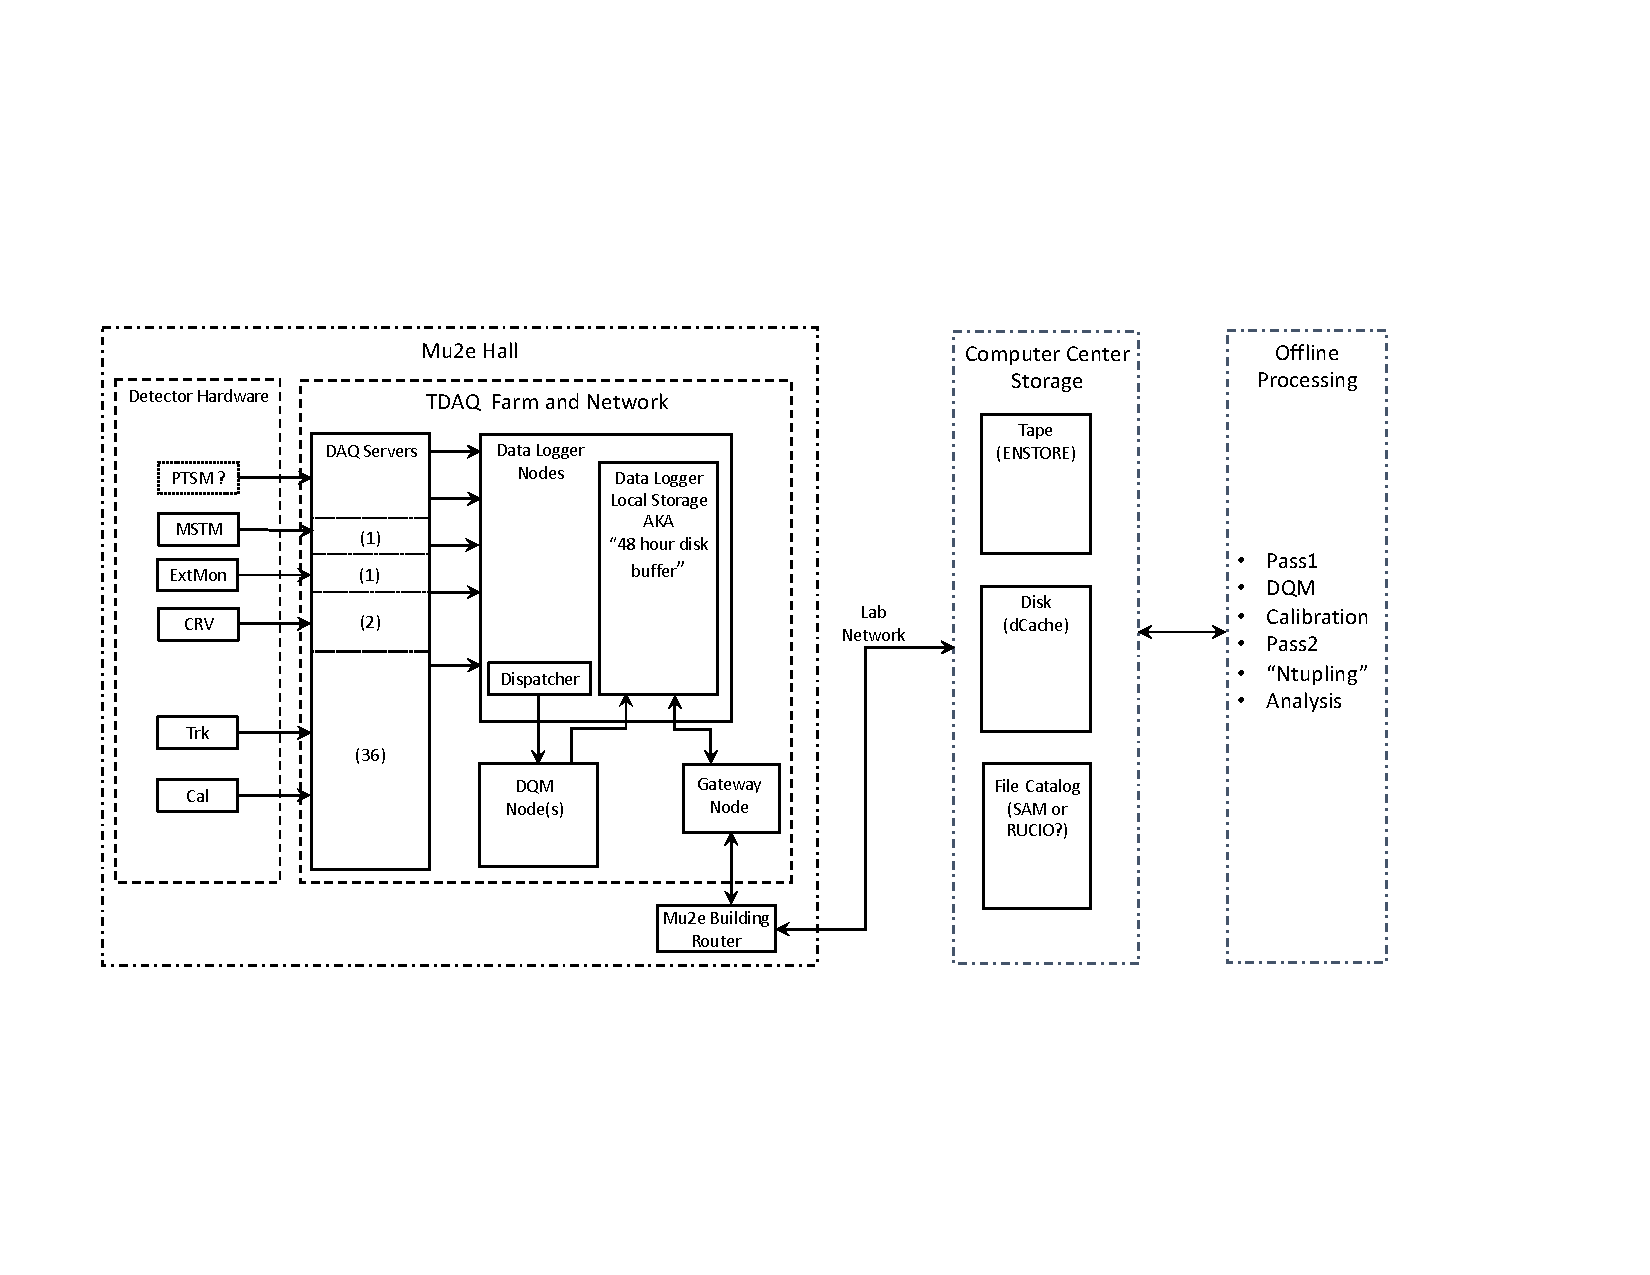
\includegraphics[width=0.9\textwidth]{figures/interface_with_TDAQ.pdf}
\caption{Block diagram of the major elements of which the Mu2e RDM must be
  aware. Not shown are \fixme{not shown}.  See the text for a discussion of these elements.}
\label{fig:blockdiagram}
\end{figure}

Data flows from the detectors, through the DAQ system into the TDAQ computer farm.
The detectors are the Tracker (Trk), Calorimeter (Cal), the Cosmic Ray Veto system (CRV),
the Muon Stopping Target Monitor (MSTM) and the downstream Extintion Monitor (ExtMon).
A sixth detector has been proposed, the Production Target Scanning Monitor (PTSM), which is
drawn with a dotted box because it is not yet funded; moreover it's primary use it to send
rapid feedback to the accelerator control room and it's not clear if it will send data
via the TDAQ system.

A cartoon picture of the farm is that it contains about 40 DAQ Server nodes
that talk to the DAQ system, build events and run trigger algorithms on those events.
Events that pass the trigger are forwarded to a Data Logger node that will write the events
to files in the ``Data Logger Local Storage'', a RAID 0 disk array on the bus of the Data Logger node.
Appendix~\ref{app:DataLoggerLocalStorage} has the specs for and a discussion about this disk array.
In earlier DPC related talks and documents this was refered to as the ``48 hour disk buffer''.
In addition to the triggered events, a variety of prescaled, untriggered events will pass the
trigger and be handled the same as events that passed the trigger.
Finally, there will be several special data streams.

The base design is to have a single data logger node that receives data from all DAQ server nodes.
Should there be limitations within the TDAQ system, such as bandwidth or latency limits,
it may be necessary to have two or more Data Logger nodes, each seeing a fraction of each data stream.
How this affects RDM will be discussed in section \fixme{add reference}.

The Data Logger nodes will also have a process called a ``Dispatcher''
that requests events from the DataLogger process
and forwards them to clients.
The Dispatcher is designed to exert no back pressure on the DataLogger process
and, therefore, will normally see only a subset of the events.
Two of the clients foreseen for the Dispatcher are an Event Display and
a Data Quality Monitoring (DQM) system,
which will produce histograms, timelines etc that can be viewed in real time.
Periodically the DQM system will write it's histograms, log files etc to
files in the data logger local storage.  One of the jobs of the RDM will be
to move these files to long term storage.

All of the computing resources in the TDAQ farm are on a private subnet
and cannot been seen from the lab network.  Access in and out
of the private subnet will be via a gateway node that is connected to
both private subnet and the lab network.  The gateway node is the responsibility
of the TDAQ group.

When the Mu2e Hall was built and provisioned, CCD personnel installed a dual router
and connected it to the lab optical fiber network.
RDM will move data from the Mu2e Hall
to the computer center using this router and the lab optical fibre network.
The router is standard item that CCD uses in many places around the lab; it stocks spares.
CCD is responsible for the maintenance of both the router and the network.
There are two M\&S items associated with the router: Mu2e pays a yearly
maintenance fee on the router and Mu2e is responsible to pay for replacement
of the router when the warrantee period expires.  Both are paid to CCD,
which has a lab-wide arrangement with the router vendor.
The specs of this router and additional details of Mu2e's arrangement with CCD
can be found in Appendix~\ref{app:RouterAndNetwork}.

Over the next few years Mu2e expects that the disk and tape services provided
by SCD will be dCache and ENSTORE.  At this writing Mu2e is using SAM as a file
catalog system.  One of the questions to ask in the design of the RDM is whether
to continue with SAM or to change to a more modern system RUCIO, which SCD
has identified as its future direction.

\chapter{The Next Chapter}
\label{ch:next_chapter}

This is chapter 2 and refers to Figure~\ref{fig:blockdiagram}



\section{If you are new to HEP Software...}

Section 1 of chapter 2


\section{If you are an HEP Software expert...}

Section 2 of chapter 2


% Keep sections under development
\IfStrEq{\ISDRAFT}{YES}{

\chapter{A Chapter under development}
\label{ch:under_development}

This is a chapter still under development

\section{If you are new to HEP Software...}

Section 1 of a chapter still under development


\section{If you are an HEP Software expert...}

Section 2 of a chapter still under development

} % end `ISDRAFT = YES'

\chapter{Requirements}

This chapter lists requirements for the RDM system.

\begin{enumerate}
  \item Move data in a timely fashion
  \item prioritize recovery from down time.
\end{enumerate}

\chapter{Questions}

A list of questions that should be addressed in the design of the RDM:

\begin{enumerate}
\item Start by sticking with SAM and move to RUCIO later?  Or move to RUCIO now?
  How does this decision interact with requirements for ongoing simulation, VST
  and test stand work?
\end{enumerate}


\appendix

\chapter{SubRuns}
\label{ch:app_Subruns}

This appendix has information about subruns

\section{If you are new to HEP Software...}

Section 1 of the appendix on subruns that refers to Table~\ref{tab:clhep:functions}.
\begin{table}
\begin{center}
\caption[Selected member functions of {\tt CLHEP::Hep3Vector}]{Selected member functions of {\tt CLHEP::Hep3Vector}.}
\label{tab:clhep:functions}
\begin{tabular}{lll}\hline
  {\cppfcl a = u.cosTheta();}  & {\cppfcl double cosTheta() const;} & $\cos\theta$\\
  {\cppfcl a = u.cos2Theta();} & {\cppfcl double cos2Theta() const;} & $\cos^2\theta$\\
  {\cppfcl v = u.unit();}      & {\cppfcl Hep3Vector unit() const;} & A unit vector in the direction of {\cppfcl u} \\ \hline
  \end{tabular}
\end{center}
\end{table}


\section{If you are an HEP Software expert...}

Section 2 of the appendix on subruns.

\chapter{Network Between Mu2e Building Router and Computer Center}
\label{app:RouterAndNetwork}.

The Mu2e building router is owned by CCD.
\begin{itemize}
\item specs; dual; auto fail over; channels; free to increase \#channels
\item Router is owned and maintained by CCD; stock item so they can replace quickly.
\item We pay yearly maintenance: \fixme{Amount in FY21 and inflation estimate}
\item We pay for replacement; we pay CCD and they do the work. \fixme{when is next replacement due; replacement cycle}
\item \fixme{make sure this is in MOU} Coverage.
\item \fixme{not sure who paid for the existing one.}
\end{itemize}


The lab network.
\begin{itemize}
\item Install and maintained by CCD.
\item Normal maintenance and repair is budgeted for in their ops budget
\item If there were an emergency repair that exceeded their budget they would come to us. \fixme{make sure this is covered in MOU}
\end{itemize}

\chapter{Data Logger Local Storage}
\label{app:DataLoggerLocalStorage}

Specs etc on the Data Logger Local Storage.


\section{If you are new to HEP Software...}

Section 1 of the appendix on subruns.


\section{If you are an HEP Software expert...}

Section 2 of the appendix on subruns.

\cleardoublepage
\printindex

